\chapter{Implementasi dan Pengujian Perangkat Lunak}
\label{chap: Implementasi dan Pengujian Perangkat Lunak}

Bab ini terdiri atas dua bagian, yaitu Implementasi Perangkat Lunak dan Pengujian Perangkat Lunak. Bagian implementasi berisi penjelasan lingkungan pengembangan perangkat lunak dan hasil implementasi. Sedangkan bagian pengujian berisi hasil pengujian fungsional terhadap perangkat lunak yang telah dibangun.

\section{Implementasi Perangkat Lunak}
\label{sec: Implementasi Perangkat Lunak}

Pada bagian ini akan dibahas mengenai implementasi perangkat lunak yang telah dibangun. Sub bab ini terdiri atas tiga bagian, yaitu lingkungan perangkat lunak, hasil implementasi perangkat lunak, dan Pengujian fungsional.

\subsection{Lingkungan Implementasi Perangkat Lunak}
\label{sec: Lingkungan Implementasi Perangkat Lunak}

Dalam proses membangun perangkat lunak ini digunakan spesifikasi perangkat sebagai berikut:

\begin{enumerate}
\item Lingkungan Pembangunan \\
\begin{itemize}
\item Processor : Intel® Core™i7-4702MQ 2.2-3.2GHz
\item RAM : 4.00 GB
\item Harddisk : 1TB
\item VGA : NVIDIA GeForce GT 740M
\item Sistem Operasi Komputer : Windows 10 Education 64-bit
\end{itemize}

\item Lingkungan Implementasi
\begin{itemize}
\item Sistem Operasi Server : \textit{Node.js}
\item Tools : \textit{Visual Studio Code}
\item Bahasa Pemrograman : Javascript
\item Framework : \textit{viz.js}
\end{itemize}

\end{enumerate}

\subsection{Hasil Implementasi}
\label{sec: Hasil Implementasi}

Kode program pada perangkat lunak ditulis dalam bahasa pemrograman \textit{javascript} dengan cara men \textit{generate} dari JSON ke \textit{DOT}. Hasil implementasi berupa pohon kurikulum yang visualisasinya menggunakan \textit{viz.js}. Perangkat lunak dapat dilihat seperti gambar \ref{fig: pohon kurikulum} di bawah ini.

\begin{figure}[H]
		\left.
		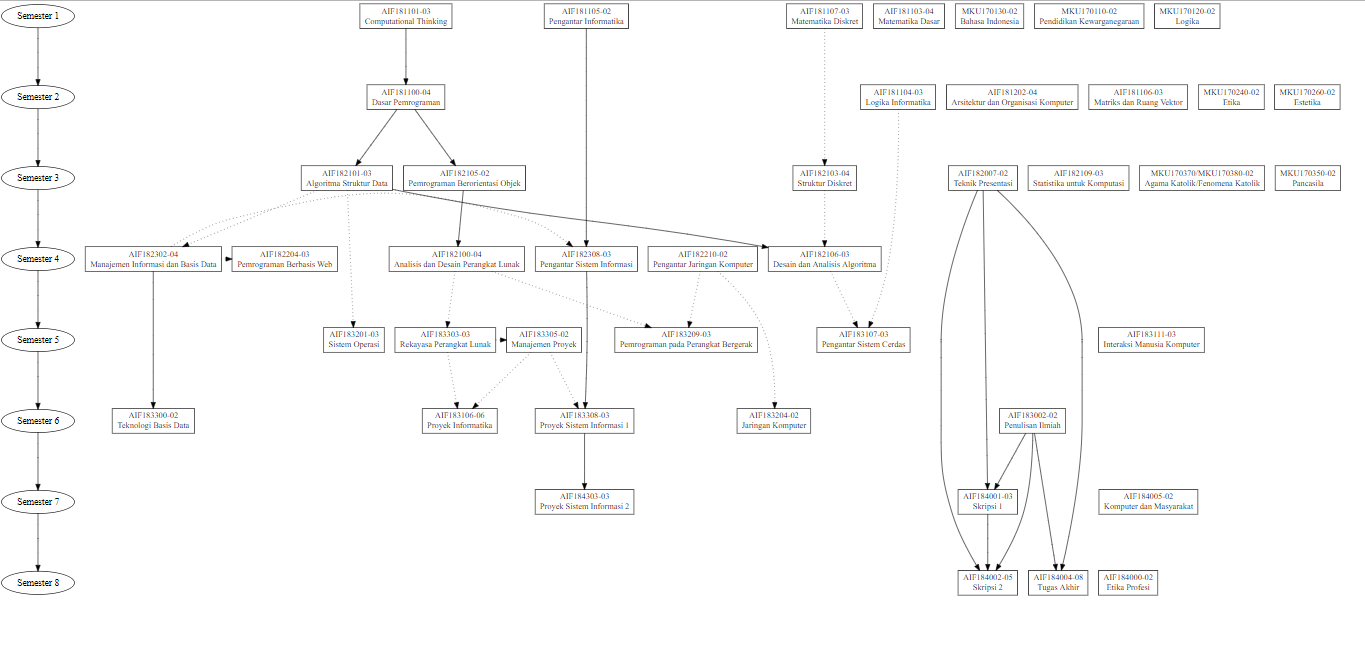
\includegraphics[scale = 0.5]{pohonkurikulum.png}
		\caption{pohon kurikulum}
		\label{fig: pohon kurikulum}
\end{figure}	 

Pada gambar \ref{fig: pohon kurikulum} terlihat setiap semester memiliki mata kuliah yang berisi kode, sks, dan nama. Lalu mata kuliah yang memiliki prasyarat akan ditunjuk oleh panah. Syarat yang menjadi patokan adalah syarat tempuh, syarat lulus, atau pengambilan secara bersamaan.
\section{Pengujian Perangkat Lunak}
\label{sec: Pengujian Perangkat Lunak}

Pada bab ini akan dibahas mengenai pengujian perangkat lunak yang dibangun. Pengujian yang dilakukan adalah pengujian fungsional. Pengujian fungsional bertujuan untuk memastikan bahwa seluruh fungsi perangkat
lunak yang dibangun berjalan sesuai dengan rencana.

\subsection{Pengujian Fungsional}
\label{sec: Pengujian Fungsional}
Dalam sub bab ini akan dilakukan pengujian fungsional untuk mengetahui fungsi-fungsi yang terdapat
pada perangkat lunak dapat berjalan sesuai dengan yang diharapkan. Status pengujian dibagi
menjadi dua yaitu "OK" dan "gagal". Di bawah ini Pengujian fungsi pohon kurikulum:

\begin{enumerate}
\item Langkah Pengujian : Memanggil fungsi rankSep   
Hal yang diharapkan : Pada saat memanggil fungsi ranksep keluar node semester dan kode mata kuliah wajib\\
Hasil Pengujian : Hasil pengujian node semester satu sampai delapan keluar dan kode mata kuliah wajib keluar \\
Status : OK\\

\item Langkah Pengujian : Memanggil fungsi nodesMatkul  
Hal yang diharapkan : Pada saat memanggil fungsi nodesMatkul akan keluar label yang berisi kode, sks, dan nama mata kuliah\\
Hasil Pengujian : & kode, sks, dan nama mata kuliah wajib berhasil ditampilkan& \\
Status : OK\\

\item Langkah Pengujian : Memanggil fungsi edgesMatkul \\
Hal yang diharapkan :  Mata kuliah yang mempunyai prasyarat bisa diketahui melalui petunjuk arah \\
Hasil Pengujian : Hasilnya mata kuliah yang memiliki prasyarat akan ditunjuk sesuai prasyarat. Jika syaratnya lulus maka garis akan lurus jika syaratnya tempuh garis putus-putus\\
Status : OK \\
